% Generated by thesis/ch7/exp2/make_assets.py -- do not edit by hand.
\begin{figure}[tbp]
  \centering
  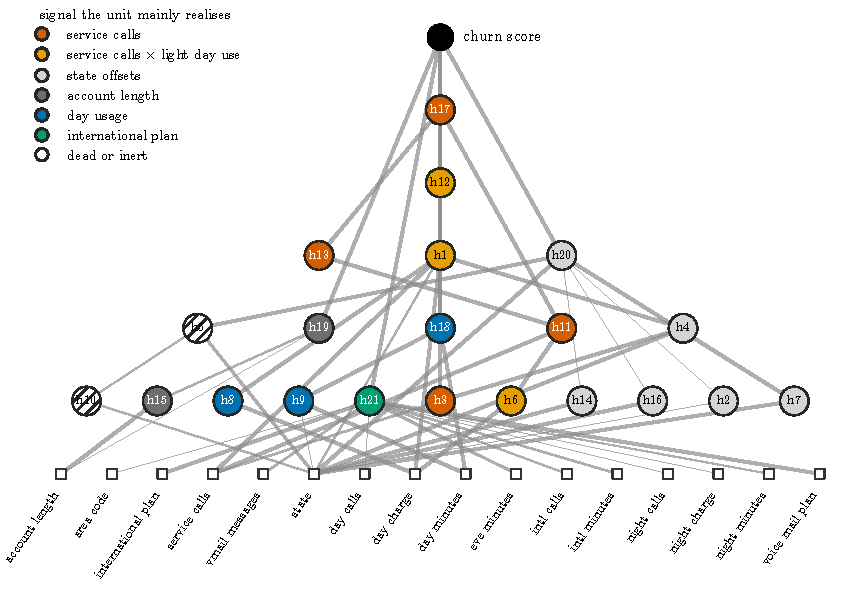
\includegraphics[width=\textwidth]{figures/exp2/exp2-churn-s5-network}
  \caption{Churn seed 5: every hidden node (21, labelled h1 to h21 as in the plain-language report) coloured by the signal it mainly realises; the 31 state indicators it reads are drawn as one input and line width follows the absolute weight. The service-call threshold and its interaction with light day use are built from 6 units (h1, h3, h6, h11, h12, h13); the identity nodes added by the explanation (h17, h18, h19, h20, h21) gather each part's output.}
  \label{fig:exp2-churn-s5-network}
\end{figure}
